\documentclass{article}

\usepackage[dblblindworkshop]{neurips_2026}
\workshoptitle{Economics for Machine Learning}

\usepackage[utf8]{inputenc}
\usepackage[T1]{fontenc}
\usepackage{hyperref}
\usepackage{url}
\usepackage{booktabs}
\usepackage{amsfonts}
\usepackage{amsmath}
\usepackage{nicefrac}
\usepackage{microtype}
\usepackage{xcolor}
\usepackage{graphicx}

\title{What Does Repairing Choice Inconsistency Buy? \\ A Budget-Set Diagnosis}

\author{%
  Anonymous Author(s) \\
  Affiliation \\
  Address \\
  \texttt{email} \\
}

\begin{document}

\maketitle

\begin{abstract}
Repairing an AI agent's incoherent preferences is an established line of work: inference-time
transitivity repairs, isotonic projections onto preference-defined cones, and training-time
rationality penalties have all been proposed, several with reported downstream gains. No published
result includes a displacement-matched control, so none establishes whether the reported gains come
from restoring coherence or from displacement toward an interior point. We build that control.
Given an LLM agent's own choices over budget sets, we compute the minimal MILP perturbation
restoring GARP-consistency, then compare it against a GARP-blind null operator spending the
identical displacement budget shrinking every bundle toward a fixed interior point. Under the first
payoff, the null outperforms the real repair by more than $2\times$ (mean $\Delta$payoff 0.0220
vs.\ 0.0091, Wilcoxon $p=3.98\times10^{-10}$, winning 81\% of traces). A second payoff built to
remove the first one's exploitable fixed target reproduces the same verdict (null 0.0217 vs.\ real
0.0072, $p=1.24\times10^{-5}$, 70.8\% win rate). Trace extremity predicts the null's advantage in
both experiments. The paper's contributions are a capacity-deconfounded identification strategy
for the coherence--competence question and a discard-selection instrument-validity finding. That
question remains open.
\end{abstract}

\section{Introduction}
\label{sec:intro}

An LLM agent asked to allocate a fixed budget across two goods at varying prices, repeatedly,
will frequently violate the Generalized Axiom of Revealed Preference (GARP;
\citealp{afriat1967construction,varian1982nonparametric}): it prefers bundle
$x_1$ to $x_2$ at one budget line and the reverse at another, in a way no monotone utility
function can rationalize. The same budget-allocation instrument is the standard paradigm for
testing GARP experimentally on human subjects \citep{andreoni2002giving,choi2007consistency,
choi2014rational}, and a growing literature applies it to GPT-family models with no repair step,
asking whether they satisfy classical rationality axioms
\citep{chen2023emergence}. A separate literature repairs this kind of inconsistency in LLM
systems --- restoring transitivity in pairwise judgments, projecting cardinal scores onto
monotone cones, and penalizing incoherence during training --- and several of these systems report
that the repaired outputs are downstream-better than the raw ones. None of them establishes
a \emph{dose}: how much better, as a function of how much repair was needed, isolated from the
capacity and training confounds that come from comparing a richer model class to a poorer one.

An LLM agent makes a
sequence of budget-constrained choices over two goods. We compute, as a single mixed-integer
linear program, the minimal quantity perturbation that would make the agent's own realized choice
sequence GARP-consistent. The projection is applied post hoc to a frozen agent: nothing
about its weights, training, or decoding changes across doses. The size of that perturbation is a
graded, cardinal dose. We score both the raw and the repaired sequence against a fixed,
equal-weight Cobb--Douglas payoff whose optimum at each budget line is a closed-form function of
prices and income alone --- never of the agent's own choices --- so the outcome measure is
exogenous to the preference data by construction.

The design does not identify the effect of coherence restoration. An operator that spends the
identical displacement budget shrinking every bundle toward a fixed interior point, with no access
to the GARP violation structure, outperforms the real GARP-restoring repair on the exogenous
payoff ($p=3.98\times10^{-10}$; \S\ref{sec:results-c1}). The result holds at both model scales and
under two payoff designs. No published axiom-enforcement result we are aware of
includes this control. Restoring GARP-consistency buys no more exogenous payoff than displacement
toward the interior of the budget line (0.0091 vs.\ 0.0220). We label this claim C1; C2 is the
coherence--competence question and C3 the claim that the reciprocal-framing manipulation disrupts
the agent.

The conjunction is new: an agent's own realized choices, a graded
coherence-indexed dose, and an outcome that is not itself a preference judgment, run together so
that dose is not confounded with model capacity or training. We run this at a model scale where the
pilot found coherence headroom (1.5B parameters), and repeat the same pipeline at 3B, where the
pilot found mean baseline CCEI 0.99. The 3B run is an identification control on the method. The two
scales are not two points on a shared dose curve.

The reciprocal-price framing manipulation
intended to induce coherence variation at 1.5B produced, in the pilot, a large apparent effect
that disappears once discard-selection is corrected with a capped retry protocol: the pilot's
uncorrected estimate and the retry-corrected estimate are both statistically indistinguishable
from zero. The discard rate is the more reliable signal that the manipulation disrupted the agent
(our claim C3): it is measured without conditioning on completion, and the CCEI point estimate is
not. The gap between the uncorrected and the corrected estimate quantifies how much a naive
discard rule can distort a measured effect (\S\ref{sec:results-framing}). Replacing single-turn
elicitation with 25 sequential calls at 1.5B drops the GARP pass rate from 0.40 to 0.10, with no
discard confound in either condition. The drop runs opposite to an independently published
finding in the same domain and model family at a larger scale \citep{wang2025tactics}.

\textbf{Contributions.} (1) An application of
\citet{demuynck2023computing}'s minimal-quantity-error MILP projection to an agent's own realized
choices, verified independently on every output, not by solver status. (2)
A closed-form exogenous payoff, fixed before any data collection, checked for leakage and for the
mechanical confound that larger violations have more room to improve. (3) A
dose-matched, GARP-blind null-operator control, run against two exogenous payoff
designs. The measured raw dose--response relationship does not show that
restoring GARP-consistency buys the exogenous payoff gain: displacement toward the interior buys
as much (\S\ref{sec:results-c1}). (4) An instrument-validity finding
(discard-selection bias under a disruptive manipulation), corrected by a capped retry
protocol and reported per cell. (5) A single-turn-vs-multi-turn elicitation-format
manipulation that drops the GARP pass rate from 0.40 to 0.10 at 1.5B. The drop runs opposite to an
independently published single-turn-vs-multi-turn finding in the same
budget-allocation domain and the same model family (Qwen2.5) at a larger scale
\citep{wang2025tactics}.

\section{Related Work}
\label{sec:related}

Four criteria jointly define the claim: an agent's own choices, an exogenous payoff, a graded
rather than binary dose, and a minimum-distance projection. Of nine published repair systems, none
satisfies all four (Table~\ref{tab:related}).

\begin{table}[h]
\centering\footnotesize
\caption{Nine published repair systems scored against the four criteria that define the claim.
\emph{Own choices}: the repaired object is a choice the agent made for itself from a budget set.
\emph{Exogenous payoff}: an outcome into which no preference judgment enters; \emph{graded dose}:
the intervention has a continuous magnitude, not an on/off setting; \emph{min.-distance
projection}: the edit is the solution to an explicit minimum-distance program.}
\label{tab:related}
\begin{tabular}{lcccc}
\toprule
& Own & Exogenous & Graded & Min.-distance \\
& choices & payoff & dose & projection \\
\midrule
POISE \citep{wang2026poise}                       & no  & no  & no  & \textbf{yes} \\
Rationality layer \citep{chadwick2025dutchbooks}  & no  & no  & no  & \textbf{yes} \\
TrustJudge \citep{wang2025trustjudge}             & no  & no  & no  & no \\
CONSISTRE \citep{sun2026consistre}                & no  & partial & no & no \\
LLM-RankFusion \citep{zeng2024rankfusion}         & no  & \textbf{yes} & no & no (declined) \\
Innate preferences \citep{buchanan2026innate}     & \textbf{yes} & no & no & no \\
GARP-EFM \citep{aguiar2026garpefm}                & no  & \textbf{yes} & no & no \\
HRC/DSPPO \citep{huang2026hrc}                    & no  & no  & \textbf{yes} & no \\
Control vectors \citep{cook2026whatllmswant}      & \textbf{yes} & no & \textbf{yes} & no \\
\midrule
This paper                                        & \textbf{yes} & \textbf{yes} & \textbf{yes} & \textbf{yes} \\
\bottomrule
\end{tabular}
\end{table}

\textbf{POISE.} \citet{wang2026poise} project with pool-adjacent-violators onto a closed convex
chain-monotone cone, and prove the edit lands weakly closer to a posited ground truth. The
GARP-consistent set is a union of polyhedra, hence not convex, so the non-expansiveness of
projection onto a closed convex set in $L_2$ does not transfer (\S\ref{app:guarantee}); the
minimum-distance priority is theirs. POISE projects a \emph{teacher's} offline labels. Three
further inference-time repairs have a binary edit and no Afriat machinery:
\citet{chadwick2025dutchbooks}, TrustJudge \citep{wang2025trustjudge}, and CONSISTRE
\citep{sun2026consistre}. LLM-RankFusion \citep{zeng2024rankfusion} has an exogenous
payoff but declines a minimum-distance method. \citet{buchanan2026innate} alters the agent itself
at training time and reports no downstream comparison. \citet{aguiar2026garpefm} is not an LLM
agent and is evaluated on forecasting.

\textbf{Preference-model variants.} A parallel line, outside the table because it varies the
transitivity of the \emph{preference model} rather than an agent's choices, makes the
cycle-tolerant arm a strict superset model class: GPM \citep{zhang2025gpm} and HRC/DSPPO
\citep{huang2026hrc}. Coherence is therefore confounded with capacity by construction, and on
GPM's own length-controlled metric that arm loses in 18 of 24 cells. HRC/DSPPO's
inverted-U dose--response curve is over a training-time schedule weight on a learned proxy, scored
by an LLM judge. Ours acts post hoc on a payoff that is exogenous by construction.
\citet{andrews2026revealed} proposes $1-\mathrm{CCEI}$ as a training penalty on a priori grounds
and reports no measurement of it. We report the measurement that proposal calls for.

\textbf{Psychometric reliability.}
\citet{nitsch2022reliability} find that CCEI and Houtman--Maks \citep{houtman1985determining}
reliability never reaches acceptable levels across eight datasets, and that mean CCEI fell among
participants given a chance to revise their own choices. Their revision arm re-presented a random
subset of trials with no consistency objective, so it could not guarantee fewer violations; ours
attains rationalizability by construction. Repair by construction rather than by re-presentation
also separates ours from \citet{yamin2026elicited}'s isotonic repair, which their own evaluation
reports as worse in 14 of 16 cells. \citeauthor{nitsch2022reliability} diagnose
their finding as a between-subject-variance problem whose prescribed remedy, a between-groups
design, is this paper's design (\S\ref{sec:limitations} bounds how far our power supports it).
Three independently published axiom-enforcement results --- \citet{nitsch2022reliability},
\citet{yamin2026elicited}, and \citet{zhu2025axiomatic} --- all report that enforcing axioms
failed to improve the outcome measured. We therefore carry a null-operator control that none of
the three had.

\textbf{Economic-choice steering.} \citet{cook2026whatllmswant}, in the economics literature,
steer economic choices toward payoff-maximizing behavior with personas and control vectors. They
meet two of the four criteria and use no Afriat machinery. They find that reframing moves models
while persona prompting does not, which corroborates our manipulation choice.
\citet{wang2025tactics} find the same in the same domain and model family (Qwen2.5) at 7B, where
collapsing multi-turn to single-turn drops CCEI by $0.241$. Which format is more degrading
reverses between their 7B model and ours: reversing their manipulation reverses the sign, and the
GARP pass rate falls from 0.40 to 0.10 (\S\ref{sec:results-multiturn}).

\section{Method}
\label{sec:method}

\subsection{Minimal-quantity-error MILP projection}
\label{sec:method-projection}

The MILP formulation below is
\citet{demuynck2023computing}'s multiplier-free ordinal characterization of minimal-quantity-error
GARP repair, applied here to an LLM agent's own choice sequence.

For a sequence of $T$ observations $(p_t, x_t)_{t=1}^T$, $K$ goods, GARP holds if there is no
sequence of choices such that $x_{t_1}$ is revealed preferred to $x_{t_2}$, \dots, $x_{t_n}$ is
revealed preferred to $x_{t_1}$, with at least one strict revealed preference in the cycle.
Given a GARP-violating sequence, we seek the minimal perturbation $\tilde{x}_t$ that restores
GARP-consistency. The Afriat-multiplier formulation is bilinear in the unknowns once
$\tilde{x}$ is itself a decision variable; we instead use the multiplier-free ordinal
characterization of \citet{demuynck2023computing}, under which every constraint is linear. At
$T=25$ and $K=2$ this is 600 binaries and 125 continuous variables per trace, solved as a single
MILP on the HiGHS backend \citep{huangfu2018parallelizing}. The full formulation and the three
method commitments are in Appendix~\ref{app:method-detail}. All 85 projections were re-verified
GARP-consistent by the Warshall-closure GARP check \citep{warshall1962theorem}, independently of
the solver (MIP gap $\le 8.1\times10^{-5}$ on every solve).

The objective is $L_1$: minimal total absolute displacement between $\tilde{x}$ and $x$ across
goods and rounds ($L_\infty$ is recorded alongside; $L_2$ would require an MIQP formulation).
Weights are uniform, which keeps the program a pure MILP. The \emph{dose} for a trace is its $L_1$
projection distance $\sum_t\sum_k |x_{t,k}-\tilde{x}_{t,k}|$ (Figure~\ref{fig:pipeline}, step 5),
comparable across sessions without further normalization because income is fixed throughout. It is
the same style of graded, minimum-cost severity measure as \citet{dean2016measuring}, applied here
to an LLM's own choices
and paired with the exogenous payoff of \S\ref{sec:method-payoff}. Wherever a mean dose or mean
$\Delta$payoff is reported over a group of traces, it is averaged over every trace in that group,
with $0$ for any already-GARP-consistent trace. We compute a Cobb--Douglas demand whose
expenditure shares are fitted to each trace's observed data as an upper bound on the reported
distance; it is not supplied to the solver (Appendix~\ref{app:payoff-audit}, check~1).

\textbf{Guarantees.} Because the GARP-consistent set is a union of polyhedra rather than a single
convex set, we claim no distance-minimization guarantee analogous to a convex-cone projection
\citep{wang2026poise}.

\subsection{The exogenous payoff}
\label{sec:method-payoff}

The payoff is fixed independently of the agent's revealed choices. A utility function fit
to the agent's choices (such as the share-fitted Cobb--Douglas demand of
\S\ref{sec:method-projection}) would be circular if used as the outcome measure, rewarding the
agent for resembling its own revealed preferences. We use an equal-weight Cobb--Douglas valuation
$U_{\mathrm{exo}}(x) = x_A^{0.5} x_B^{0.5}$, fixed before any model was queried. It was never
re-estimated from any agent's choices. At budget line $(p_t, I_t)$ the optimal bundle
$x^*_t$ is the closed-form Cobb--Douglas demand $x^*_{t,A}=0.5 I_t/p_{t,A}$,
$x^*_{t,B}=0.5 I_t/p_{t,B}$, which depends only on prices and income. The payoff score is the
efficiency ratio
$\mathrm{payoff}(x_t) = U_{\mathrm{exo}}(x_t)/U_{\mathrm{exo}}(x^*_t) \in (0,1]$, computed
identically for the raw and projected sequence at the same budget lines, so that
$\Delta\mathrm{payoff} = \mathrm{payoff}(\tilde{x}) - \mathrm{payoff}(x)$ is comparable across
conditions, models, and repairs. This has the structure of a
money-metric utility index, the standard welfare-comparison device over the same GARP/Afriat
objects this paper's method already relies on. \citet{ouyang2024aidecisionmaker} give one of the
few comparable exogenous, real-world payoffs: they score LLM-generated forecasts
against firms' realized future spending and find a \emph{non-monotonic} alignment-accuracy
relationship. Separating an alignment-specific effect from a generic fine-tuning effect requires a
placebo of matched size, which that design lacks. Our design makes that separation.

We checked four failure modes of this design: a shared-data leak between payoff and projection, a
mechanical link between GARP-consistency and payoff, a projection direction correlated with the
payoff optimum, and the confound that larger-dose traces start with lower payoff and have more
room to improve. All four are ruled out --- the fourth, the strongest of them, leaves the dose
coefficient significant once raw payoff is controlled for (Appendix~\ref{app:payoff-audit} gives
every check and number) --- so the raw dose--response statistic of \S\ref{sec:results-c1} is not
attributable to any of them. A fifth concern, that this payoff's concavity could reward
displacement alone, motivates the control constructed next.

\subsection{Null-operator controls}
\label{sec:method-nullop}

The payoff of \S\ref{sec:method-payoff} reduces to $\mathrm{payoff}(s)=2\sqrt{s(1-s)}$, where $s$
is the expenditure share on good A. It is concave with a single interior maximum at $s=0.5$,
identical across every trace. Any operator that moves a bundle toward that fixed point raises that
bundle's payoff whether or not it restores GARP-consistency. We construct a \emph{null operator}
that shrinks every observed bundle in a GARP-violating trace toward the exogenous optimum $x^*_t$
by a single shared factor $\lambda\in[0,1]$, chosen so the null's total $L_1$ displacement exactly
matches the real projection's dose. The null does not call the GARP check and is not guaranteed to
restore consistency; it is scored by the payoff of \S\ref{sec:method-payoff}.

Because that fixed target is identical across every trace, we build a
second payoff that removes it: a per-trace Cobb--Douglas weight
$\alpha_s\sim\mathrm{Uniform}(0.05,0.95)$, drawn independently for each of the 85 traces and each
of $K=20$ replicate draws, read only at scoring time. We report two null constructions under this
payoff: a \emph{primary} null, unaware of $\alpha_s$, and an
\emph{oracle} null that aims at the true per-trace optimum $x^*_{\alpha_s}$. The two are reported
separately. The oracle null is an upper bound: it uses the per-trace $\alpha_s$, which a repair
algorithm does not observe.

\begin{figure}[t]
  \centering
  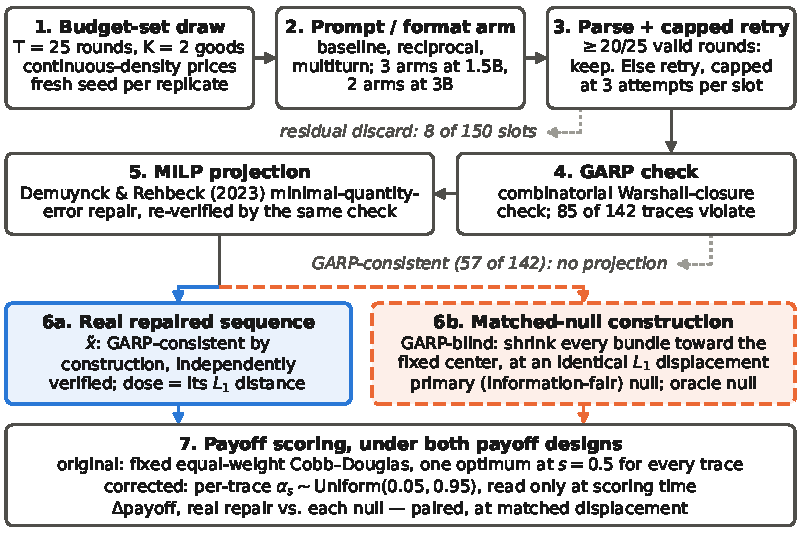
\includegraphics[width=0.98\linewidth]{../figures/fig_pipeline_schematic.pdf}
  \caption{The pipeline, one replicate end to end: budget-set draw (1); prompt/format condition
  (2); parse (3); GARP check (4); and, for the traces that violate it, the
  minimal-quantity-error MILP of \S\ref{sec:method-projection} (5). The real repaired sequence
  (6a, solid blue) and the GARP-blind null spending an identical $L_1$ displacement (6b, dashed
  orange) are scored (7) under both payoff designs.}
  \label{fig:pipeline}
\end{figure}

\section{Experimental design}
\label{sec:design}

\subsection{Models and conditions}

We use two locally hosted open-weight models: \texttt{qwen2.5:1.5b-instruct} at 1.5B and
\texttt{llama3.2:3b-instruct} at 3B. The pilot found within-condition coherence variation at 1.5B
and mean baseline CCEI 0.99 at 3B, so 1.5B carries the dose--response measurement and 3B serves as
a low-headroom control. Models were run one at a time, all runs for one model completing before
the next was loaded; concurrent residency of a third model family caused reproducible crashes.
\textbf{Compute.} All inference ran locally on 4-bit-quantized weights, with no GPU and no
commercial API calls. The full $N=30$ design completed in $\approx$2.1 hours wall-clock, every
MILP projection (\S\ref{sec:method-projection}) solving in under 5 seconds.

Three conditions at 1.5B, two at 3B. \textbf{Baseline.} Direct per-token-return framing, single
turn, all 25 rounds in one prompt and response. \textbf{Reciprocal.} The same single-turn format
with an inverted-price framing manipulation, the strongest manipulation identified in the pilot.
\textbf{Multi-turn} (1.5B only). Baseline framing, but each of the 25 rounds is a separate
sequential call carrying the running conversation history, which isolates the elicitation-format
mechanism from the price-framing mechanism. \citet{wang2025tactics} collapse multi-turn to
single-turn in the same domain and find that this drops CCEI by $0.241$ for a same-family model at
7B; because our baseline is already single-turn, this condition tests the reverse. The 3B model is
a low-headroom control, so this condition was run at 1.5B only.

\subsection{Budget sets and power}

Each of $N=30$ independent replicates per (model, condition) cell draws a fresh $T=25$,
$K=2$ budget set (prices $p_A,p_B\sim U[0.1,1.0]$ i.i.d., rejected unless
$\max(p_A,p_B)\ge0.5$, budget exhaustion enforced), seeded independently. Independent seeding
supports between-condition replication. A \emph{slot} is one such design position; each slot is run
for up to three \emph{attempts}, one session each (\S\ref{sec:discard}); a completed attempt yields
one \emph{trace}.
Continuous, independently drawn prices with enforced budget exhaustion also avoid a
pathology documented by \citet{andrews2026revealed}: CCEI can read exactly 1.0 on GARP-violating
data whenever a comparison lands on exact budget-line equality, common under grid-sampled or
rounded prices.
$N=30$ gives power $\ge0.999$ against the pilot's full framing-effect magnitude on the pass-rate
metric and $\ge0.80$ down to $\sim$60\% attenuation, but is underpowered for a
CCEI-scale effect of the pilot's magnitude at 1.5B (minimum detectable $\approx0.11$). Every
replicate's Bronars power of the budget set \citep{bronars1987power} is recorded;
all 150 draws held Bronars power $\ge0.998$.

\subsection{Discard selection and the retry protocol}
\label{sec:discard}

The pilot found that under reciprocal framing at 1.5B, 52\% of sessions (13 of 25) failed the
required output format and were silently discarded under the pilot's handling. Silent discarding
is standard practice; this paper measures its consequences. This is a claim
about instrument validity. The main experiment implements a capped retry protocol: a session
failing the $\ge20/25$-valid-rounds threshold is retried up to three times with a new random seed;
a slot still failing after three attempts is a residual discard, excluded from the main CCEI/GARP
analysis but scored separately for the audit in Table~\ref{tab:discardbreakdown}. Three of the 30
qwen reciprocal slots returned zero valid rounds on all three attempts, yielding no price or
quantity data.

At 1.5B, retry-rescued sessions differ from first-attempt sessions: mean CCEI 0.9651 against
0.9315, but GARP pass rate 0.1429 against 0.4706. The residual-discard group has the lowest mean
CCEI of the three (0.8821), though its GARP pass rate is measured on only 3 slots. The residual
sample is too small ($n=6$, 3 measurable) to be conclusive, but the pattern is consistent with the
pilot's selection concern surviving the retry correction at reduced magnitude. At 3B, the
first-attempt and retry-rescued groups differ by 0.0118 in CCEI and 0.143 in GARP pass rate, so
the selection concern shows up more sharply at 1.5B than at 3B.

\begin{table}[h]
\centering
\footnotesize
\caption{Discard-outcome breakdown for all 60 reciprocal-framing sessions (30 per model), by
attempt group: kept on the first attempt, rescued by a later retry, or still discarded after three
attempts (\S\ref{sec:discard}). GARP pass, CCEI and mean dose ($L_1$) follow the conventions of
\S\ref{sec:method-projection} and Table~\ref{tab:headline}. $^*$Computed over the 3 of 6 qwen
residual-discard slots with any valid rounds.}
\label{tab:discardbreakdown}
\begin{tabular}{llrrrr}
\toprule
Model & Attempt group & $n$ & mean CCEI & GARP pass & mean dose ($L_1$) \\
\midrule
llama3.2:3b  & first-attempt success & 21 & 0.9742 & 0.4286 & 5.086 \\
llama3.2:3b  & retry-rescued         & 7  & 0.9624 & 0.2857 & 9.839 \\
llama3.2:3b  & residual discard      & 2  & 1.0000 & 1.0000 & 0.000 \\
\midrule
qwen2.5:1.5b & first-attempt success & 17 & 0.9315 & 0.4706 & 13.847 \\
qwen2.5:1.5b & retry-rescued         & 7  & 0.9651 & 0.1429 & 7.600 \\
qwen2.5:1.5b & residual discard      & 6  & 0.8821$^*$ & 0.6667$^*$ & 24.196$^*$ \\
\bottomrule
\end{tabular}
\end{table}

\section{Results}
\label{sec:results}

We ran 150 slots (llama3.2:3b in 2 conditions, qwen2.5:1.5b in 3, 30 replicates each)
and made 187 attempts. Of these, 142 slots kept a usable trace and 8 were residual discards after
three attempts. Every cell was run to its full 30 slots.

\begin{table}[t]
\caption{Headline results per (model, condition) cell. GARP pass and CCEI are computed on kept
traces only; dose and $\Delta$payoff are averaged over all kept traces, with $0$ for any
already-GARP-consistent trace, and are under the original payoff (\S\ref{sec:method-payoff}).}
\label{tab:headline}
\centering
\footnotesize
\begin{tabular}{llrrrrr}
\toprule
Model & Condition & $n$ kept & mean CCEI & GARP pass & mean dose ($L_1$) & mean $\Delta$payoff \\
\midrule
llama3.2:3b  & baseline   & 30 & 0.9900 & 0.73 & 5.01  & +0.0018 \\
llama3.2:3b  & reciprocal & 28 & 0.9713 & 0.39 & 6.27  & +0.0016 \\
qwen2.5:1.5b & baseline   & 30 & 0.9522 & 0.40 & 16.68 & +0.0090 \\
qwen2.5:1.5b & multi-turn & 30 & 0.9540 & 0.10 & 14.54 & +0.0083 \\
qwen2.5:1.5b & reciprocal & 24 & 0.9413 & 0.38 & 12.02 & +0.0065 \\
\bottomrule
\end{tabular}
\end{table}

\subsection{Dose--response and the null-operator control}
\label{sec:results-c1}

Across the 85 GARP-violating traces (60 at
1.5B, 25 at 3B): Spearman $\rho=0.729$ ($p<0.0001$), Pearson $r=0.821$ ($p<0.0001$), mean
$\Delta$payoff $+0.0091$ (one-sample $t=5.41$, $p<0.00001$), with 70 of 85 traces (82\%) improving
after repair and 15 (18\%) worsening. The relationship holds at each scale separately:
$\rho=0.756$ ($p<0.0001$, $n=60$) at 1.5B and $\rho=0.614$
($p=0.0011$, $n=25$) at 3B. We do not compare its magnitude across scale. We tested the mechanical
confound that larger-dose traces might start from worse raw payoff and therefore have more room to
improve. The confound is real (dose
vs.\ raw payoff, Pearson $r=-0.41$, $p<0.0001$) but does not explain the relationship away. The
partial correlation of dose against $\Delta$payoff controlling for raw payoff is $r=0.784$
($p=7\times10^{-19}$). An OLS regression of $\Delta$payoff on dose and raw payoff jointly
finds dose significant ($t=11.4$, $p<10^{-16}$), with raw payoff's marginal contribution
not distinguishable from zero ($p=0.18$) once dose is included
(Appendix~\ref{app:payoff-audit}).

\begin{figure}[t]
  \centering
  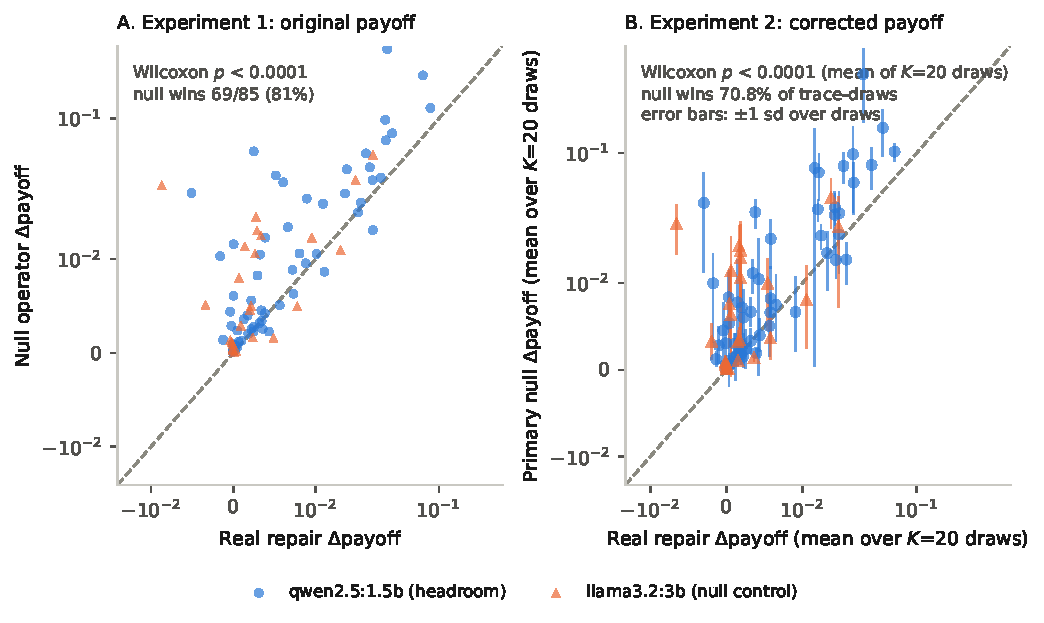
\includegraphics[width=0.76\linewidth]{../figures/fig1_dose_response.pdf}
  \caption{Real repair's $\Delta$payoff (x-axis) against the dose-matched null operator's
  $\Delta$payoff (y-axis) on symmetric-log axes, one point per GARP-violating trace ($n=85$;
  circle/blue: qwen2.5:1.5b, triangle/orange: llama3.2:3b). Dashed line is $y=x$; points above it
  have higher null $\Delta$payoff than real. \textbf{(A)} Experiment 1, original payoff;
  \textbf{(B)} Experiment 2, corrected payoff, with each trace's primary-null $\Delta$payoff
  averaged over $K=20$ draws of the random target ($\pm1$ SD error bars).}
  \label{fig:doseresponse}
\end{figure}

The raw-payoff confound bears on the \emph{severity} of the raw violation. It leaves open whether
restoring GARP-consistency or the displacement does the work. The null operator
(\S\ref{sec:method-nullop}) spends the identical $L_1$ budget as the real repair and shrinks every
bundle toward the exogenous payoff's fixed optimum, using no GARP information.

\textbf{Experiment 1 (original payoff).} The null operator outperforms the real repair by
$2.4\times$: mean $\Delta$payoff$_{\mathrm{null}}=0.0220$ vs.\ mean
$\Delta$payoff$_{\mathrm{real}}=0.0091$, Wilcoxon signed-rank $p=3.98\times10^{-10}$, with the
null winning 69 of 85 traces (81\%; Fig.~\ref{fig:doseresponse}A). This holds at both model
scales. The partial correlation of dose against $\Delta$payoff$_{\mathrm{real}}$, controlling for
the null's mechanically predicted gain, remains positive and significant ($r=0.574$,
$p=1.13\times10^{-8}$), so dose retains information beyond what the null predicts.

\textbf{Experiment 2 (corrected payoff).} The original payoff's exploit is a single fixed target
($s=0.5$) identical across every trace. Experiment 2 draws an independent Cobb--Douglas weight
$\alpha_s\sim\mathrm{Uniform}(0.05,0.95)$ per trace, over $K=20$ independent draws
(\S\ref{sec:method-nullop}). Experiment 2 reproduces Experiment 1: the primary null still
outperforms the real repair, by $3.0\times$ (mean
$\Delta$payoff$_{\mathrm{null}}=0.02167$ vs.\ mean $\Delta$payoff$_{\mathrm{real}}=0.00723$,
Wilcoxon $p=1.24\times10^{-5}$, win rate 70.8\%), significant in 20 of 20 draws. The oracle null,
privileged to know the true per-trace target, wins 80.4\% of traces (mean
$\Delta$payoff$_{\mathrm{null}}=0.02224$, $p=1.35\times10^{-9}$, significant in 20 of 20 draws).
The partial correlation of dose with $\Delta$payoff$_{\mathrm{real}}$, controlling for the null,
attenuates from Experiment 1's $r=0.574$ to a mean $r=0.37$ across the 20 draws, significant in
14--15 of 20.

\textbf{Two payoff designs.} One is the paper's original; the second was built to remove the
first one's exploitable structure. Both return the same negative paired comparison. A third
payoff, selected after seeing that the second was also negative, would be payoff-shopping
(\S\ref{sec:limitations}).

\textbf{Trace extremity and the null's advantage.} Trace extremity ($1-\text{raw payoff}$ under
the original fixed payoff, a measure of the raw bundles independent of which payoff later scores
them) predicts the null's advantage in both experiments (Experiment 1: Pearson $r=0.679$;
Experiment 2 primary null: mean $r=0.631$ across 20 draws), and predicts the real repair's own
gain less strongly in both. This pattern does not separate ``centering'' from a
more general account on which moving an extreme trace toward the interior helps regardless of
destination, since Experiment 2's primary null is mechanically the same fixed-center operator as
Experiment 1's. Experiment 2's oracle null, which targets a per-trace-varying
point, shows the same extremity-advantage to within 0.01 (mean $r=0.624$ against 0.631). We treat
the ``escape a bad start'' reading as a hypothesis for the discussion; we do not test it.
Figure~\ref{fig:mechanism} illustrates it on a single trace. On the largest-dose trace the repair
changes 5 of 21 rounds, spending 42\% of its $L_1$ budget on round 3 alone ($s$
$0.11\!\to\!0.65$, payoff $0.626\!\to\!0.953$) and leaving the other 16 at a near-corner $s=0.99$,
while the null spreads the same total displacement over all 21 rounds.

\begin{figure}[t]
  \centering
  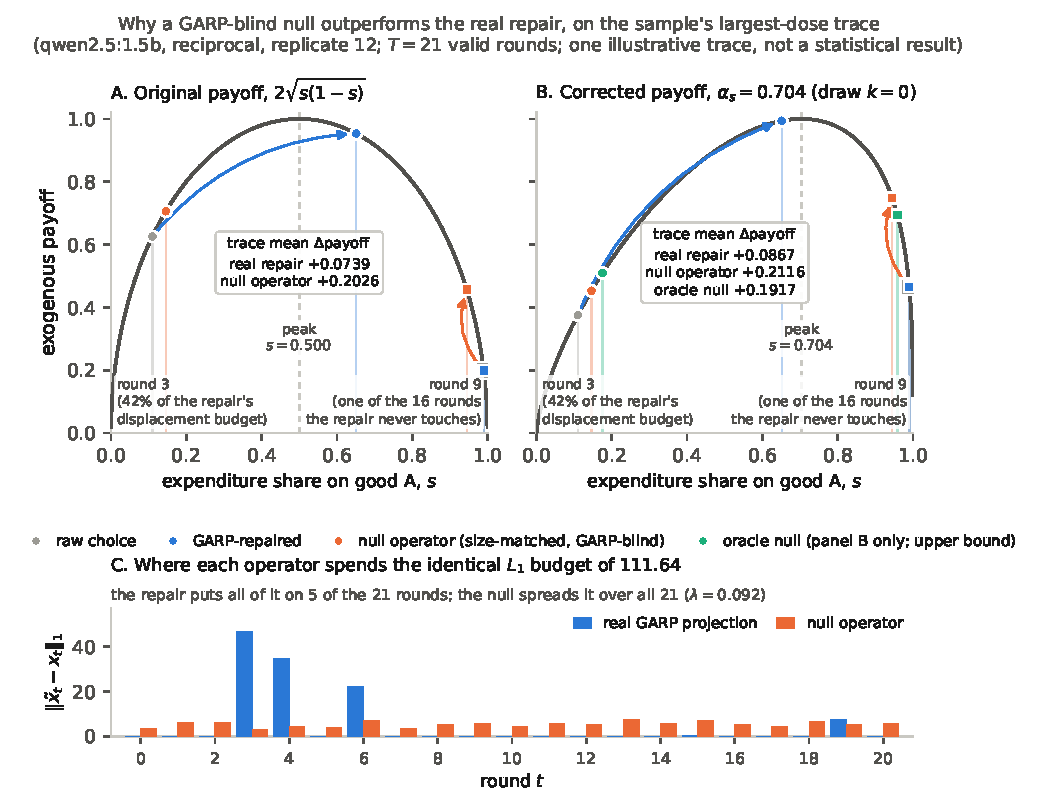
\includegraphics[width=0.98\linewidth]{../figures/fig_mechanism_illustration.pdf}
  \caption{The largest-dose trace (qwen2.5:1.5b, reciprocal, replicate 12; $L_1=111.64$,
  $T=21$ rounds). With $K=2$, payoff is a function of expenditure share $s$.
  \textbf{(A)} The original payoff $2\sqrt{s(1-s)}$, peak at $s=0.5$;
  \textbf{(B)} the corrected payoff at this trace's draw $\alpha_s=0.704$;
  \textbf{(C)} per-round $s$ across all 21 rounds for the raw
  trace, the real repair, and the null operator.}
  \label{fig:mechanism}
\end{figure}

The hypothesis that restoring GARP-consistency, beyond displacement toward the interior of the
budget line, buys more exogenous payoff (C1) is not supported under either payoff design. The raw
dose--response relationship holds; it is not evidence for the specific mechanism C1 claims.

\subsection{Reciprocal framing and discard selection}
\label{sec:results-framing}

At 3B, reciprocal framing replicates the pilot's finding on an independently drawn budget set:
GARP pass rate drops from 0.73 (22/30) to 0.39 (11/28), $p=0.0089$ (Benjamini--Hochberg
$p_{\mathrm{BH}}=0.011$, Holm $p_{\mathrm{Holm}}=0.062$); CCEI does not reach significance
(0.9900 vs.\ 0.9713, $t$-test $p=0.0508$). CCEI compresses near 1, as the pilot found. Here, GARP
pass rate separated baseline from reciprocal and CCEI did not.

At 1.5B, the reciprocal-framing effect does not survive
correction for discard-selection. First-attempt discard under reciprocal framing was 43.3\%
(13/30), against the pilot's unretried 52\%, falling to a residual 20.0\% (6/30) after the retry
protocol. Reciprocal framing produces more discards than
any other condition, including the other 1.5B manipulation (multi-turn, 0\%). Once the
surviving 24 sessions are compared, GARP pass rate (0.40 vs.\ 0.38, $p=0.85$) and CCEI (0.9522
vs.\ 0.9413, $p=0.73$) are indistinguishable between baseline and reciprocal framing. Neither
experiment detects a CCEI shift: the pilot's $+0.0169$
($p=0.66$) and the main experiment's $-0.0109$ ($p=0.73$) are two statistically indistinguishable
nulls.
Table~\ref{tab:discardbreakdown} breaks the discards down by attempt.

\subsection{Multi-turn elicitation format}
\label{sec:results-multiturn}

Replacing the single prompt with 25 sequential calls drops the GARP pass rate from 40\% to
10\% ($p=0.0073$) while CCEI does not move (0.9522 vs.\ 0.9540, $p=0.91$;
Table~\ref{tab:multiturn}), with zero discards in either condition. Reciprocal framing produced no
detectable drop at 1.5B, so the multi-turn format is the only 1.5B manipulation with a measured
pass-rate effect. The drop survives Benjamini--Hochberg correction ($p_{\mathrm{BH}}=0.0094$) but
not Holm ($p_{\mathrm{Holm}}=0.058$). Together with the 3B reciprocal-framing result
(\S\ref{sec:results-framing}), GARP pass rate again separates the conditions and CCEI does not.
\citet{wang2025tactics} report the opposite: in the same domain, on the same model
family at 7B (Qwen2.5-7B), single-turn elicitation was more coherence-degrading
than multi-turn; here, at 1.5B, the reverse holds. We have no explanation for the reversal.

\begin{table}[h]
\centering
\footnotesize
\caption{1.5B (qwen2.5:1.5b), baseline vs.\ multi-turn elicitation format (25 sequential calls),
$n=30$ per condition. GARP pass rate is reported as count/$n$ with 95\% Wilson score confidence
intervals (Pearson $\chi^2$ test, $p=0.0073$); mean CCEI is reported with 95\% $t$-based
confidence intervals ($df=29$; two-sample $t$-test, $p=0.91$).}
\label{tab:multiturn}
\begin{tabular}{lccc}
\toprule
Condition & GARP pass & 95\% CI (Wilson) & mean CCEI [95\% CI ($t$)] \\
\midrule
baseline                    & 12/30 (40.0\%) & [24.6, 57.7]\% & 0.9522 [0.9253, 0.9791] \\
multi-turn (25 seq.\ calls) & 3/30 (10.0\%)  & [3.5, 25.6]\%  & 0.9540 [0.9350, 0.9729] \\
\bottomrule
\end{tabular}
\end{table}

\section{Limitations}
\label{sec:limitations}

\textbf{CCEI is underpowered at 1.5B.} The 1.5B model's within-condition CCEI noise (baseline
WSCV 14.8\%) is comparable to published human test--retest noise on the same index
\citep{nitsch2022reliability}, and $N=30$ is underpowered for a CCEI-scale effect of the pilot's
magnitude: the minimum detectable effect is $2.5\times$ the pilot's estimate. A CCEI-power-matched
design would need $N=111$--$161$; we did not run that design. The pass-rate metric is powered
$\ge0.999$ throughout, and every CCEI result carries its own confidence interval.

\textbf{Single run per condition.} Every (model, condition) cell is one
run of the stated protocol. There are no repeated full-pipeline runs, so we report no between-run
variance on the headline pass-rate and $\Delta$payoff statistics, only the within-run replicate
variance in the reported confidence intervals and $p$-values.

\textbf{One scale point per model.} The two-model design isolates the identification
strategy from a scale confound but does not trace a dose--response relationship \emph{across}
scale. In our model-selection sweep (\S\ref{sec:design}), coherence headroom and measurement
reliability did not coexist in any model tested, and a third model family was excluded because it
could not be run alongside the others.

\textbf{Two exogenous payoffs.} We report two payoff designs
(\S\ref{sec:method-payoff}, \S\ref{sec:method-nullop}). The first payoff's single, globally
identical optimum is exploitable by a GARP-blind operator; the second removes that property and
reproduces the same verdict. A third payoff, selected after seeing that the second was also
negative, would be payoff-shopping, which is the researcher-degree-of-freedom problem an exogenous
payoff was introduced to rule out (\S\ref{sec:results-c1}).

\textbf{Consistent with three prior negative results.} Three independently
published repair attempts moved the wrong way (\S\ref{sec:related}). The null-operator result of
\S\ref{sec:results-c1} is a fourth: under two payoffs, restoring GARP-consistency does not
outperform a dose-matched GARP-blind operator. Separately, our reciprocal-framing manipulation at
1.5B (\S\ref{sec:results-framing}) failed to induce the coherence variation it was designed to
induce. Net of displacement, this paper's attempt to find a positive coherence--competence
relationship did not succeed. That leaves C2 open; it is not evidence that the relationship is
negative in general.

\section{Broader Impacts}

This paper's result argues against imposing GARP repair on AI economic agents as a routine
intervention applied without a matched control: under two payoff designs, a GARP-blind operator
that displaces choices toward an interior point outperforms the real repair
(\S\ref{sec:results-c1}). A practitioner deploying coherence repair on the strength of a raw
within-scale dose--response correlation alone would be acting on the confounded estimate this
paper's control was built to separate. Correcting the discard selection removes the
reciprocal-framing manipulation's apparent effect on the coherence it was designed to disrupt
(\S\ref{sec:results-framing}). The design measures whether repair helps. Here it does not. The
discard-selection finding (\S\ref{sec:discard}) is not specific to our instrument: a consistency
instrument that drops disruption-caused failures without recording them will underestimate the
disrupting manipulation. We see no elevated misuse risk specific to this work: synthetic
tasks, open-weight models, no new dataset, no human subjects.

\section{Conclusion}
\label{sec:conclusion}

Restoring GARP-consistency in an LLM agent's own realized choices does not buy more exogenous
payoff than displacement alone. Applying the minimal-quantity-error GARP repair of
\citet{demuynck2023computing} post hoc to a frozen agent, we find a monotone raw within-scale
dose--response relationship between dose and $\Delta$payoff. At both model scales and under two
payoff designs, a dose-matched, GARP-blind null operator outperforms the real repair on that same
payoff ($p=3.98\times10^{-10}$ and $p=1.24\times10^{-5}$). C1 is not supported.

Trace extremity predicts the null's advantage in both experiments, which offers a candidate
explanation for that advantage but does not establish it. The paper's identification argument
(C2) survives: the coherence--competence relationship remains open, and this is the first attempt
we know of to measure it without confounding coherence with capacity, a preference-judgment
outcome, or displacement magnitude. A practitioner evaluating coherence repair should include a
dose-matched null operator before reading a dose--response correlation as evidence of benefit.

Two further findings stand on their own. A framing manipulation's apparent effect was a
discard-selection artifact (C3). An elicitation-format manipulation moved GARP pass rate in the
direction opposite to that reported by \citet{wang2025tactics}, in the same domain and model
family at a larger scale.

\begin{ack}
\end{ack}

\bibliographystyle{plainnat}
\bibliography{references}

\appendix

\section{Payoff exogeneity audit}
\label{app:payoff-audit}

\textbf{(1) Payoff inputs.} The payoff is computed from $(p_t, I_t)$ by a routine that reads no
projection output; the optimal bundle $x^*_t$ is a function of
$(p_t, I_t)$ alone and never references $x_t$ or $\tilde{x}_t$. The share-fitted Cobb--Douglas
demand of \S\ref{sec:method-projection} is used only to log an upper bound on the reported
distance. It is never passed to HiGHS as an incumbent solution, for which the solver exposes no
interface.

\textbf{(2) Independence of the payoff optimum from revealed preference.} Raw (pre-repair) payoff
does not differ between the 57 already-GARP-consistent traces and the 85 violating traces
(0.7872 vs.\ 0.7899; Welch $t=-0.07$, $p=0.94$). No population-level link between GARP-consistency
and payoff is detectable.

\textbf{(3) Trace-level mechanism check.} Five traces spanning the dose range (0.17 to
111.64) were inspected by hand, comparing the direction of the actual projection movement
$(\tilde{x}-x)$ against the direction toward the exogenous optimum $(x^*-x)$ via cosine
similarity; every quantity plotted in Figure~\ref{fig:mechanism} was recomputed by re-solving the
projection MILP. Similarities were low (0.16--0.31) on the four traces where payoff improved after
repair, and negative ($-0.35$) on the single trace where payoff worsened. On these five traces the
sign of the cosine similarity matched the sign of the payoff change, and the cosine of the
projection step against $(x^*-x)$ appears nowhere in the projection objective. This is evidence
against the projection acting as a disguised optimization toward the payoff target.

\textbf{(4) Severity confound.} Larger-dose traces start from worse raw payoff
(Pearson $r=-0.41$, $p<0.0001$), and worse-starting traces improve more
($r=-0.41$ between raw payoff and $\Delta$payoff). This is a ceiling-effect confound. The
dose--response relationship survives it: the partial correlation of dose against
$\Delta$payoff controlling for raw payoff is $r=0.784$ ($p=7\times10^{-19}$). The unconditional
correlation is $r=0.821$. In a joint OLS regression the dose coefficient is
significant ($t=11.43$, $p<10^{-16}$) while raw payoff's coefficient is not
($t=-1.36$, $p=0.18$).

No part of the audit found a channel by which the projection could influence payoff other than
through $(p_t, I_t)$.

\section{MILP formulation and implementation}
\label{app:method-detail}

\textbf{Formulation.} We use the multiplier-free ordinal characterization of
\citet{demuynck2023computing}, under which every constraint is linear jointly in the perturbed
bundles, a set of ordinal utility levels $u_t\in[0,1]$, and binary comparison indicators
$U_{t,v}\in\{0,1\}$ for $t\neq v$. The formulation is solved as a single MILP, with no outer
search over preference orderings. Afriat-multiplier parameterizations are bilinear once
$\tilde{x}$ is a decision variable, and remain so under any fixed preference ordering, because a
price-weighted multiplier term stays a product of two unknowns.

\textbf{Budget exhaustion.} Budget exhaustion is imposed as an equality,
$p_t \cdot \tilde{x}_t = I_t$ for every observation, with income fixed at 100 throughout. The
big-$M$ constant in the ordering constraints is therefore fixed a priori: any $M > 100$ is valid,
and it needs no tuning.

\textbf{Strict-preference margin.} The GARP-consistent set is not closed, so an unregularized
projection can read a distance of exactly zero on violating data. A fixed strict-preference margin
$\gamma > 0$, set to $10^{-4}\cdot I = 10^{-2}$, converts an unattained infimum into an attained
minimum. The reported distance is stable across
$\gamma \in \{10^{-2}, 10^{-3}, 10^{-4}, 10^{-5}, 10^{-6}\}$, a sweep that runs downward from the
operating point.

\textbf{Independent verification.} Every returned $\tilde{x}$ is verified by the
Warshall-closure \citep{warshall1962theorem} GARP check of \S\ref{sec:method-projection}. All 85
GARP-violating traces' projections were re-verified GARP-consistent; MIP gap
$\le 8.1\times10^{-5}$ on every solve.

\textbf{Objective.} $\min \sum_t\sum_k w_{t,k} d_{t,k}$ subject to
$\tilde{x}_{t,k}-x_{t,k}\le d_{t,k}$ and $x_{t,k}-\tilde{x}_{t,k}\le d_{t,k}$, with uniform weights
$w=1$.

\subsection{Scope of the guarantee}
\label{app:guarantee}

The closest published analogue is a proved-optimal projection onto a convex monotone cone
\citep{wang2026poise}. There, non-expansiveness licenses a guarantee that the edit lands weakly
closer to ground truth, because the cone is fixed by an ordering supplied as input. The
GARP-consistent set is
a union of polyhedra rather than a single convex set, and a GARP repair must itself decide which
revealed-preference comparisons to give up. That decision is absorbed into the binary comparison
indicators $U_{t,v}$ rather than eliminated, so we claim no distance-minimization guarantee.

\newpage
\input{checklist.tex}

\end{document}
